\documentclass[conference,10pt]{IEEEtran}
\usepackage{amsmath,amssymb,booktabs,graphicx,microtype,url}
\usepackage[caption=false,font=footnotesize]{subfig}
\hfuzz=1pt
\title{Minority-to-Majority Incremental Class Learning on Two Imbalanced Data Sets}
\author{\IEEEauthorblockN{JW Moolman}
\IEEEauthorblockA{Student number: 26892154\\
Stellenbosch Department of Computer Science\\Module: RW741\\
Repository: \url{PLACEHOLDER HTTPS REPOSITORY URL}}}

\begin{document}
\maketitle

\begin{abstract}
The investigation evaluated minority-to-majority class presentation on the Dry Bean and Steel Plates Faults datasets. Five outer folds and fold-specific training and validation splits protected test observations during model selection. Fixed incremental learning exceeded its update-budget control by 0.0007 and 0.0047 in test Macro-F1 on Dry Bean and Steel Plates, respectively. Dynamic incremental learning exceeded dynamic all-classes by 0.0011 and 0.0037. Every primary 95\% confidence interval included zero, and no Holm-adjusted test established a reliable difference. Fixed incremental learning achieved the highest overall and minority-class means. Dynamic methods used approximately two to five hidden units on average but required more gradient updates and achieved lower absolute Macro-F1 than the fixed methods. Five overlapping training partitions limited inference.
\end{abstract}
\begin{IEEEkeywords}class imbalance, curriculum learning, incremental learning, dynamic neural networks\end{IEEEkeywords}

\section{Introduction}
Class imbalance complicates multiclass evaluation. Frequent classes dominate aggregate accuracy under severe imbalance~\cite{he2009learning}. Minority-to-majority presentation offers a possible way to change learning priorities. The investigation evaluated the resulting classification performance and the cost of validation-triggered network growth.

The first research question concerned the predictive effect of minority-first presentation. The second research question concerned the performance--size trade-off produced by dynamic growth. Dry Bean~\cite{koklu2020multiclass} and Steel Plates Faults~\cite{buscema2010steel} supplied two naturally imbalanced seven-class problems from the University of California Irvine Machine Learning Repository.\footnote{University of California Irvine Machine Learning Repository: \url{https://archive.ics.uci.edu/}} Their different sample sizes and class-imbalance ratios provided two contrasting settings for the same experimental protocol; results from two datasets were not treated as evidence of broad generality.


\section{Background}

\subsection{Imbalance and Evaluation}
Previous research showed a coincidence between high accuracy and weak rare-class performance~\cite{he2009learning}. A class-specific F1 score is the harmonic mean of precision and recall. Macro-averaged F1 score averages the class-specific F1 scores and assigns equal weight to every class~\cite{sokolova2009systematic}. The investigation selected macro-averaged F1 score as the primary measure. Minority performance was defined fold-specifically as the mean F1 score and mean recall of the two least frequent classes in that fold's inner-training partition, so the minority identities could differ between folds.

\subsection{Ordered and Sequential Learning}
Curriculum-learning research showed that presentation order affected optimisation and generalisation~\cite{bengio2009curriculum}. Continual-learning research identified interference between earlier and later tasks as a central sequential-learning problem~\cite{parisi2019continual}. The present method retained training examples from earlier classes after each introduction. The method was therefore a cumulative staged curriculum, rather than a strict continual-learning protocol with unavailable past examples. The continual-learning literature supplied context for sequential interference without describing an identical data-access setting.

\subsection{Dynamic Capacity}
Research on dynamically expandable networks showed that structural growth supported changing learning demands~\cite{yoon2018den}. The implemented growth rule used validation behaviour as an operational underfitting test. With the canonical settings in Table~\ref{tab:hyperparameters}, stagnation meant that validation macro-averaged F1 failed to improve by at least 0.001 for 10 epochs. Stagnation triggered a 15-epoch single-neuron probe; the additional unit was retained only when validation Macro-F1 improved by at least 0.001. Rejected probes still contributed to the recorded optimisation cost.


\section{Implementation}
The classifier contains a direct linear path and a nonlinear hidden path. For input vector $\boldsymbol{x}$, the logit vector $\boldsymbol{a}$ is
\begin{equation}
 \boldsymbol{a}=\boldsymbol{W}\boldsymbol{x}+\boldsymbol{b}+
 \boldsymbol{W}_{2}f(\boldsymbol{W}_{1}\boldsymbol{x}+\boldsymbol{b}_{1}),
\end{equation}
where $\boldsymbol{W}$ denotes the direct-path weight matrix, $\boldsymbol{b}$ denotes the direct-path bias vector, and $f$ denotes the rectified linear activation function. Matrices $\boldsymbol{W}_{1}$ and $\boldsymbol{W}_{2}$ contain the incoming and outgoing hidden weights. Vector $\boldsymbol{b}_{1}$ contains the hidden biases.

The residual design differs from a conventional hidden-only multilayer perceptron. A newly added hidden unit receives randomly initialised incoming weights and zero bias, while its outgoing weights are initialised to zero; the expansion therefore leaves the network function unchanged until subsequent optimisation. Output expansion retains all existing output parameters, initialises the new direct-path output weights randomly, and initialises the new bias and hidden-to-output parameters to zero. Adam moments persist while parameter shapes remain unchanged. Structural expansion changes parameter-array shapes, so the optimiser state is reset after each output or hidden-layer expansion rather than reusing moments with incompatible shapes.

Mini-batch Adam minimises cross-entropy with $L_2$ regularisation on the weight matrices. For $N$ training examples, the objective is
\begin{equation}
 \mathcal{L}=-\frac{1}{N}\sum_{i=1}^{N}\log p_{i,y_i}
 +\frac{\lambda}{2}\sum_{\boldsymbol{W}\in\mathcal{W}}\lVert\boldsymbol{W}\rVert_F^2,
\end{equation}
where $\mathcal{W}$ contains the direct and, when present, hidden-layer weight matrices. Validation macro-averaged F1 controls checkpointing and stagnation. Table~\ref{tab:hyperparameters} lists the canonical optimisation and growth settings.

\begin{table}[t]
\caption{Canonical hyperparameters}
\label{tab:hyperparameters}\centering
\begin{tabular}{lr}\toprule
Setting & Value\\\midrule
Optimiser and activation & Adam and rectified linear\\
Learning rate and batch size & 0.01 and 128\\
Maximum epochs and patience & 150 and 10\\
Minimum stopping improvement & 0.001\\
Regularisation coefficient & $10^{-4}$\\
Probe epochs and minimum gain & 15 and 0.001\\
Hidden-unit candidates & 0, 1, 2, 4, \ldots, 512\\
Optimisation seeds and outer folds & 5 and 5\\\bottomrule
\end{tabular}
\end{table}


\section{Empirical Process}
Exact duplicate rows were removed before partitioning so that identical observations could not be assigned to different training, validation, and test partitions; Table~\ref{tab:data} summarises the resulting datasets. Five stratified outer folds each reserved approximately 20\% of the data as a disjoint test partition. Within the remaining 80\%, a stratified 18.75\% holdout supplied validation data, giving approximately 65\% training, 15\% validation, and 20\% test data overall in each outer fold.

Numerical features were standardised using statistics estimated from the inner-training partition only. For feature $j$,
\begin{equation}
 x'_{ij}=\frac{x_{ij}-\mu_j}{\sigma_j},
\end{equation}
where $\mu_j$ and $\sigma_j$ are the inner-training mean and standard deviation. The same fitted transformation was then applied unchanged to validation and outer-test observations. Class-frequency order, architecture selection, early stopping, and growth decisions likewise used inner training and validation data only.

\begin{table}[t]
\caption{Data after duplicate removal}
\label{tab:data}\centering
\resizebox{\columnwidth}{!}{\begin{tabular}{lrrrrrr}\toprule
Dataset & $n$ & Features & Classes & Min. class & Max. class & Ratio\\\midrule
Dry Bean & 13543 & 16 & 7 & 522 & 3546 & 6.79\\
Steel Plates & 1941 & 27 & 7 & 55 & 673 & 12.24\\\bottomrule
\end{tabular}}
\end{table}

Architecture candidates were evaluated with five optimisation seeds on every inner validation partition. Let $F^{*}$ denote the highest mean validation macro-averaged F1 score. The selected hidden size was the smallest scalar $h$ satisfying
\begin{equation}
 F(h)\geq F^{*}-0.001,
\end{equation}
where $F(h)$ denotes the mean validation macro-averaged F1 score for hidden size $h$. The tolerance favoured the simpler model when the measured difference did not exceed 0.001. The search included capacities through 512 hidden units.

Five methods were evaluated. Within an outer fold, the ordinary baseline, fixed incremental method, and fixed update-budget control all used the same fold-selected hidden-layer size. The ordinary baseline exposed all classes from the start. The fixed incremental method instead began with the two least frequent inner-training classes and added the remaining classes from least to most frequent while retaining all previously introduced training examples. For every fold--seed pair, the fixed control exposed all classes from the start but was trained for exactly the total number of gradient updates consumed by its paired fixed incremental run. The optimiser, learning rate, batch size, regularisation, preprocessing, and selected architecture were otherwise shared, so this comparison controlled the update budget while changing the class-presentation schedule.

Dynamic all-classes and dynamic incremental both started with zero hidden units and used the same fold-selected architecture size as their maximum permitted capacity. They shared the same stagnation, single-neuron probe, gain threshold, optimiser, validation, and capacity-limit rules. Dynamic all-classes exposed every class immediately, whereas dynamic incremental used the cumulative minority-to-majority schedule; class availability was therefore the designed difference in this control pair. After stagnation, an accepted probe remained in the model and training continued on the same active-class stage, permitting further probes; a rejected probe ended capacity growth for that stage and the curriculum advanced to the next class.

The validation-only sensitivity experiment applied to dynamic incremental learning and used probe lengths of 10, 15, and 25 epochs. The gain thresholds were 0.0005, 0.001, and 0.002. All five inner splits and a single fixed seed contributed to the sensitivity experiment. Outer test outcomes did not contribute to sensitivity decisions.

The five optimisation seeds were first averaged within each outer fold. The five resulting fold means formed the paired observations for inference. For each contrast, a two-sided paired Student $t$-test was applied to those five fold means. The unadjusted 95\% confidence interval for the mean paired difference was
\begin{equation}
 \bar{d}\pm t_{0.975,\,4}\frac{s_d}{\sqrt{5}},
\end{equation}
where $\bar{d}$ and $s_d$ are the mean and sample standard deviation of the five paired fold differences. The primary family contained fixed incremental minus the fixed update-budget control and dynamic incremental minus dynamic all-classes, separately for each dataset. The corresponding minority Macro-F1 comparisons formed an exploratory family. Holm correction was applied separately to the two raw $p$-values in each reported family; the confidence intervals themselves were not multiplicity-adjusted. Tables~\ref{tab:dry-bean-statistics} and~\ref{tab:steel-plates-statistics} report $d_z=\bar{d}/s_d$. Overlapping outer-training partitions and only five test folds limited inferential precision.


\section{Results and Discussion}

\subsection{Class Imbalance}
Steel Plates exhibited stronger class imbalance than Dry Bean (Table~\ref{tab:data}; Fig.~\ref{fig:distribution}). Experimental class order and minority identities were nevertheless determined separately from each inner-training partition; the highlighted full-dataset minority classes in Fig.~\ref{fig:distribution} are therefore descriptive rather than a substitute for the fold-specific ordering.
\begin{figure*}[t]\centering
\subfloat[Dry Bean]{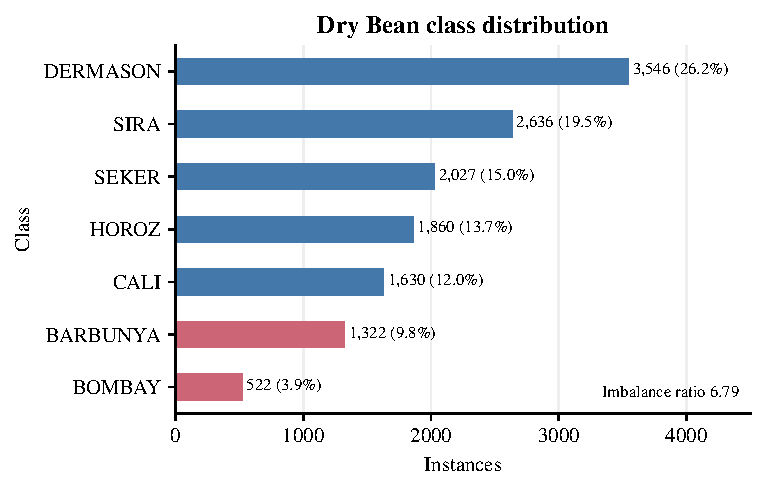
\includegraphics[width=.47\textwidth]{figures/dry_bean/class_distribution.pdf}}\hfill
\subfloat[Steel Plates Faults]{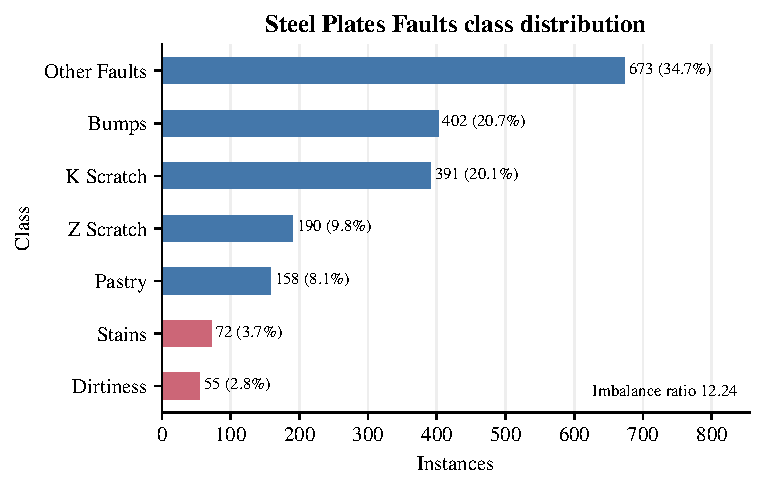
\includegraphics[width=.47\textwidth]{figures/steel_plates/class_distribution.pdf}}
\caption{Class counts after duplicate removal, sorted from least to most frequent. Labels show counts and percentages; the two minority classes are highlighted. Each panel states its largest-to-smallest class ratio. Experimental class order was determined separately within each training fold.}\label{fig:distribution}
\end{figure*}

\subsection{Architecture Selection}
Figure~\ref{fig:architecture} shows the fold-specific validation curves and selected capacities. Steel Plates folds four and five selected the maximum tested capacity, so their optima were not bracketed; 512 is therefore the best tested size for those folds rather than an established interior optimum.
\begin{figure*}[t]\centering
\subfloat[Dry Bean]{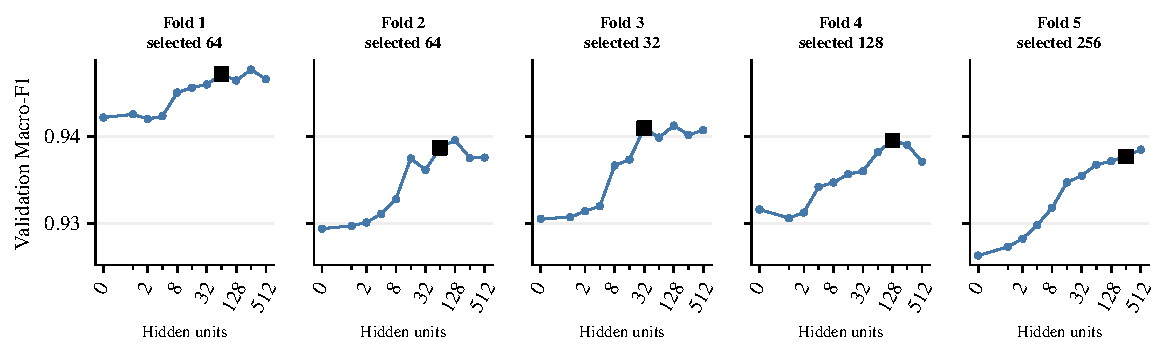
\includegraphics[width=.86\textwidth]{figures/dry_bean/baseline_architecture.pdf}}\\
\subfloat[Steel Plates Faults]{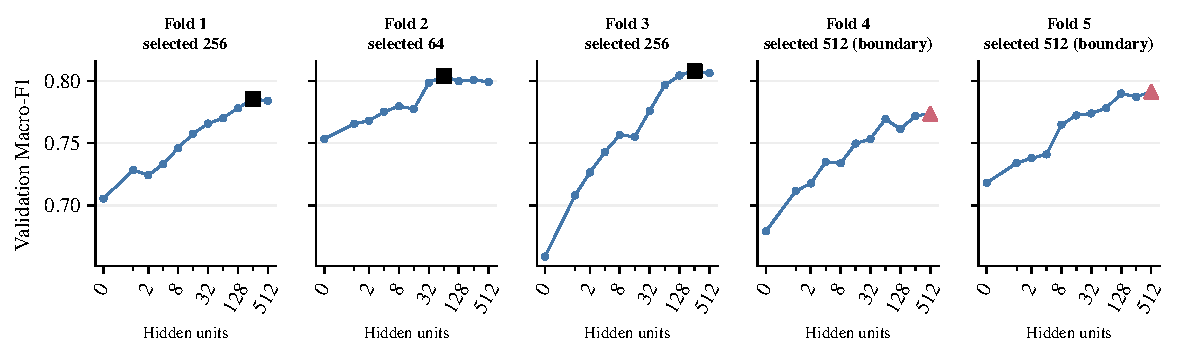
\includegraphics[width=.86\textwidth]{figures/steel_plates/baseline_architecture.pdf}}
\caption{Validation Macro-F1 across tested hidden capacities, shown separately for each outer fold. The larger marker identifies the selected size; triangles identify selections at the maximum tested capacity, which do not establish an interior optimum.}\label{fig:architecture}
\end{figure*}

\subsection{Overall Classification Performance}
\begin{table}[t]
\caption{Overall test performance: Dry Bean}
\label{tab:dry-bean-overall}
\centering
\begin{tabular}{lcc}
\toprule Method & Macro-F1 & Fold std. dev.\\
\midrule
Ordinary baseline & 0.9396 & 0.0069\\
Fixed update-budget control & 0.9405 & 0.0061\\
Dynamic all-classes & 0.9375 & 0.0063\\
Dynamic incremental & 0.9386 & 0.0064\\
Fixed incremental & 0.9412 & 0.0060\\
\bottomrule
\end{tabular}
\end{table}
\begin{table}[t]
\caption{Overall test performance: Steel Plates Faults}
\label{tab:steel-plates-overall}
\centering
\begin{tabular}{lcc}
\toprule Method & Macro-F1 & Fold std. dev.\\
\midrule
Ordinary baseline & 0.7638 & 0.0067\\
Fixed update-budget control & 0.7673 & 0.0070\\
Dynamic all-classes & 0.7312 & 0.0114\\
Dynamic incremental & 0.7348 & 0.0096\\
Fixed incremental & 0.7721 & 0.0075\\
\bottomrule
\end{tabular}
\end{table}

Fixed incremental learning had the highest observed mean Macro-F1 on both datasets, whereas the dynamic methods had lower absolute means (Tables~\ref{tab:dry-bean-overall} and~\ref{tab:steel-plates-overall}). These absolute rankings do not isolate the effect of presentation order; the paired controls below do.

\subsection{Controlled Curriculum Effects}
\begin{table*}[t]
\caption{Paired fold-level comparisons: Dry Bean}
\label{tab:dry-bean-statistics}
\centering\small
\resizebox{\textwidth}{!}{\begin{tabular}{llrrrrrr}
\toprule Family & Comparison & Mean diff. & 95\% interval & $d_z$ & Raw $p$ & Holm $p$ & $n$\\
\midrule
Primary & Fixed incremental minus Fixed update-budget control & +0.0007 & [-0.0012, 0.0026] & 0.449 & 0.3725 & 0.3725 & 5\\
Primary & Dynamic incremental minus Dynamic all-classes & +0.0011 & [-0.0002, 0.0024] & 1.069 & 0.0752 & 0.1503 & 5\\
Minority exploratory & Fixed incremental minus Fixed update-budget control & +0.0014 & [-0.0015, 0.0044] & 0.606 & 0.2471 & 0.2471 & 5\\
Minority exploratory & Dynamic incremental minus Dynamic all-classes & +0.0013 & [-0.0005, 0.0031] & 0.878 & 0.1211 & 0.2422 & 5\\
\bottomrule
\end{tabular}}
\end{table*}
\begin{table*}[t]
\caption{Paired fold-level comparisons: Steel Plates Faults}
\label{tab:steel-plates-statistics}
\centering\small
\resizebox{\textwidth}{!}{\begin{tabular}{llrrrrrr}
\toprule Family & Comparison & Mean diff. & 95\% interval & $d_z$ & Raw $p$ & Holm $p$ & $n$\\
\midrule
Primary & Fixed incremental minus Fixed update-budget control & +0.0047 & [-0.0096, 0.0191] & 0.411 & 0.4105 & 0.8210 & 5\\
Primary & Dynamic incremental minus Dynamic all-classes & +0.0037 & [-0.0094, 0.0167] & 0.350 & 0.4781 & 0.8210 & 5\\
Minority exploratory & Fixed incremental minus Fixed update-budget control & +0.0069 & [-0.0194, 0.0331] & 0.324 & 0.5091 & 0.5091 & 5\\
Minority exploratory & Dynamic incremental minus Dynamic all-classes & +0.0151 & [-0.0157, 0.0459] & 0.608 & 0.2456 & 0.4913 & 5\\
\bottomrule
\end{tabular}}
\end{table*}

Both controlled comparisons had positive mean differences on both datasets, but every primary 95\% interval crossed zero and the Holm-adjusted tests did not establish a reliable curriculum effect (Tables~\ref{tab:dry-bean-statistics} and~\ref{tab:steel-plates-statistics}; Fig.~\ref{fig:primary-effects}). The fold-level spread in Fig.~\ref{fig:primary-effects} also shows that the direction and magnitude of the effect were not consistent across folds.
\begin{figure*}[t]\centering
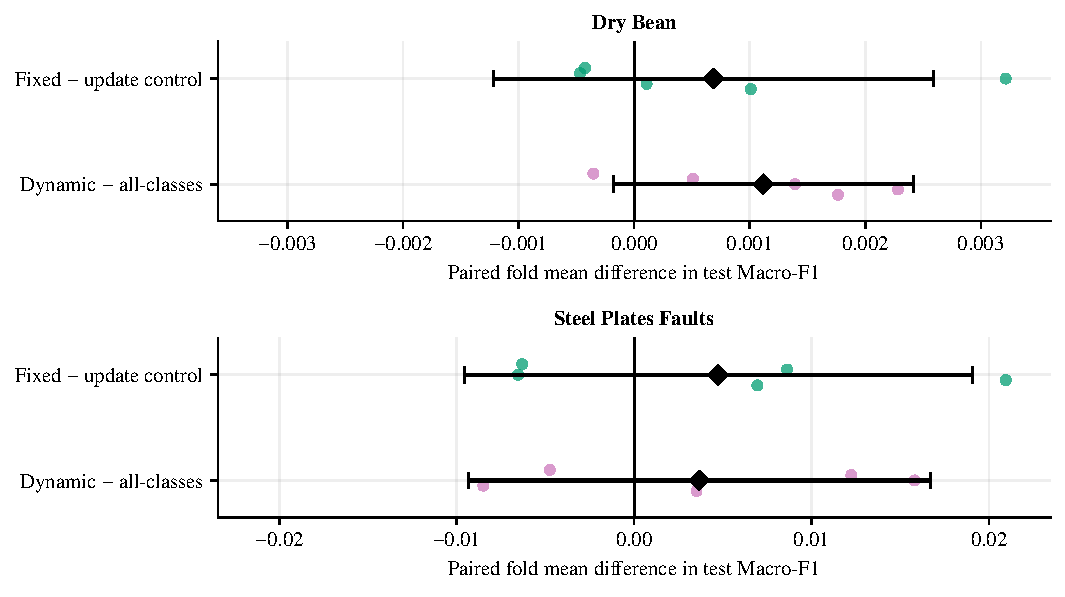
\includegraphics[width=.85\textwidth]{figures/primary_effects.pdf}
\caption{Primary paired test Macro-F1 differences. Small points show the five outer-fold differences after averaging optimisation seeds within each fold. Diamonds show mean paired differences; horizontal bars show unadjusted 95\% confidence intervals. The vertical zero line denotes no observed curriculum effect.}\label{fig:primary-effects}
\end{figure*}

\subsection{Minority and Per-Class Behaviour}
\begin{table}[t]
\caption{Minority performance: Dry Bean}
\label{tab:dry-bean-minority}
\centering
\begin{tabular}{lcc}
\toprule Method & Macro-F1 & Recall\\
\midrule
Ordinary baseline & 0.9657 & 0.9596\\
Fixed update-budget control & 0.9674 & 0.9631\\
Dynamic all-classes & 0.9633 & 0.9561\\
Dynamic incremental & 0.9646 & 0.9585\\
Fixed incremental & 0.9688 & 0.9639\\
\bottomrule
\end{tabular}
\end{table}
\begin{table}[t]
\caption{Minority performance: Steel Plates Faults}
\label{tab:steel-plates-minority}
\centering
\begin{tabular}{lcc}
\toprule Method & Macro-F1 & Recall\\
\midrule
Ordinary baseline & 0.8320 & 0.8226\\
Fixed update-budget control & 0.8438 & 0.8313\\
Dynamic all-classes & 0.7644 & 0.7794\\
Dynamic incremental & 0.7795 & 0.7934\\
Fixed incremental & 0.8506 & 0.8558\\
\bottomrule
\end{tabular}
\end{table}

Fixed incremental also had the highest observed minority Macro-F1 means, but the exploratory paired intervals for both fixed and dynamic comparisons crossed zero (Tables~\ref{tab:dry-bean-minority}--\ref{tab:steel-plates-minority} and Tables~\ref{tab:dry-bean-statistics}--\ref{tab:steel-plates-statistics}). The class-level effects were heterogeneous rather than uniformly positive: in the Steel Plates fixed comparison, Pastry showed the largest positive mean shift while Other Faults was slightly negative (Fig.~\ref{fig:per-class-effects}). No class-specific significance claim was made.
\begin{figure*}[t]\centering
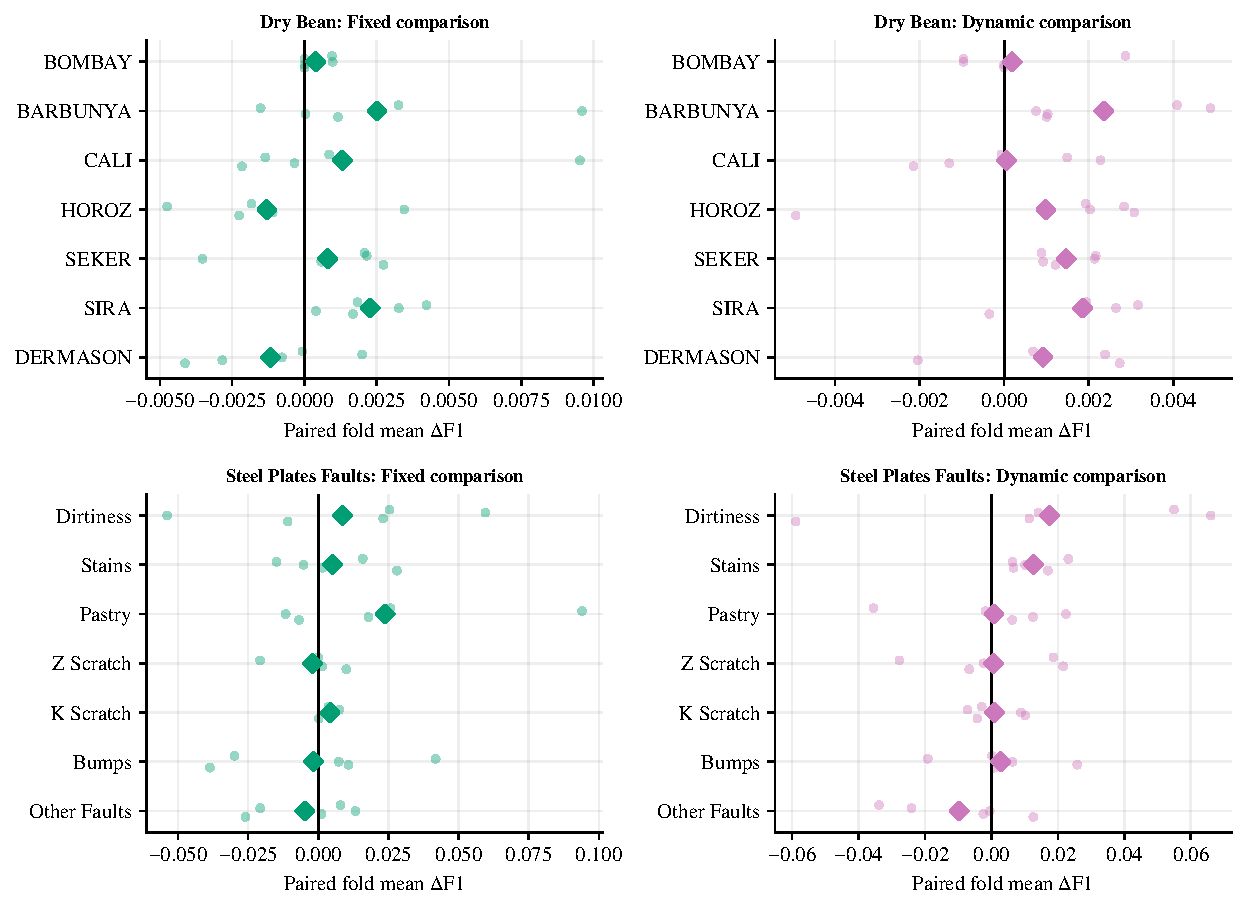
\includegraphics[width=.92\textwidth]{figures/per_class_effects.pdf}
\caption{Descriptive paired class-level test F1 differences for fixed incremental minus its update control and dynamic incremental minus dynamic all-classes. Small points are five outer-fold differences after seed averaging; diamonds are their means. Classes follow full-dataset frequency from rarest at top to most common at bottom; experimental order remained fold-specific. Zero denotes no observed class-level difference.}\label{fig:per-class-effects}
\end{figure*}

\subsection{Dynamic-Capacity Behaviour}
Validation Macro-F1 generally declined as additional classes entered the cumulative task, with substantial fold variation on Steel Plates (Fig.~\ref{fig:progression}). After the initial two-class stage, the fixed incremental mean generally remained above the dynamic incremental mean, especially on Steel Plates, while the dynamic model increased its hidden capacity as more classes became active (Figs.~\ref{fig:progression} and~\ref{fig:growth}). This shows that the growth rule reacted to the expanding task rather than remaining static, but the added capacity did not close the validation-performance gap to the fixed-capacity model. Dynamic incremental networks also finished larger than the dynamic all-classes control and incurred more accepted and rejected probes (Fig.~\ref{fig:growth}; Tables~\ref{tab:dry-bean-efficiency} and~\ref{tab:steel-plates-efficiency}). Figure~\ref{fig:dynamic-capacity-performance} shows the corresponding run-level relationship between final capacity and test Macro-F1; because capacity is produced by the growth procedure, this association is descriptive rather than causal.
\begin{figure*}[t]\centering
\subfloat[Dry Bean]{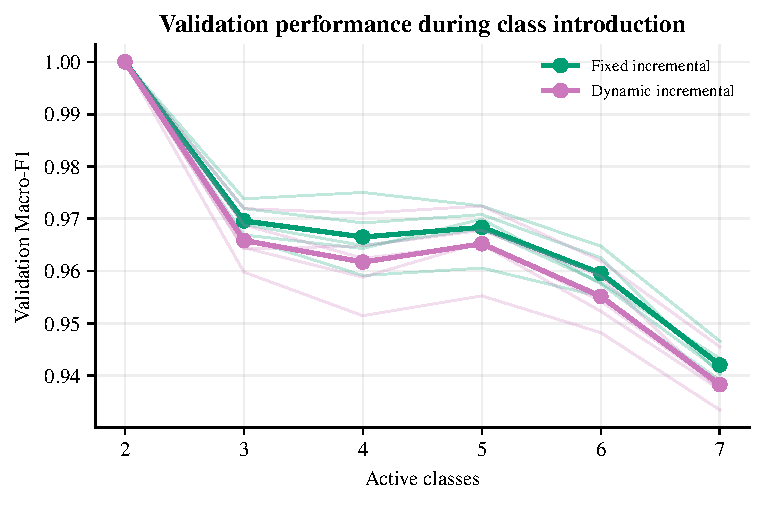
\includegraphics[width=.47\textwidth]{figures/dry_bean/incremental_progression.pdf}}\hfill
\subfloat[Steel Plates Faults]{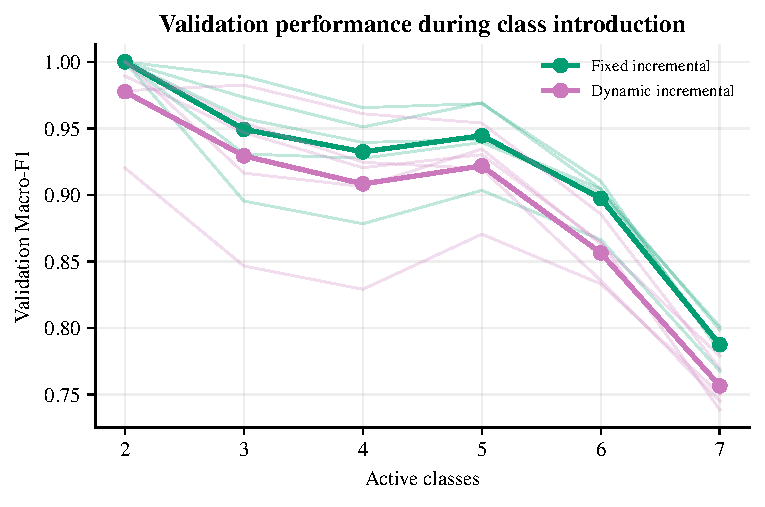
\includegraphics[width=.47\textwidth]{figures/steel_plates/incremental_progression.pdf}}
\caption{Validation Macro-F1 during cumulative class introduction. Thin lines show five outer-fold trajectories after averaging five optimisation seeds within each fold; thick lines show their mean. The task gains a class at each stage, so scores across stages are not like-for-like test comparisons.}\label{fig:progression}
\end{figure*}
\begin{figure*}[t]\centering
\subfloat[Dry Bean]{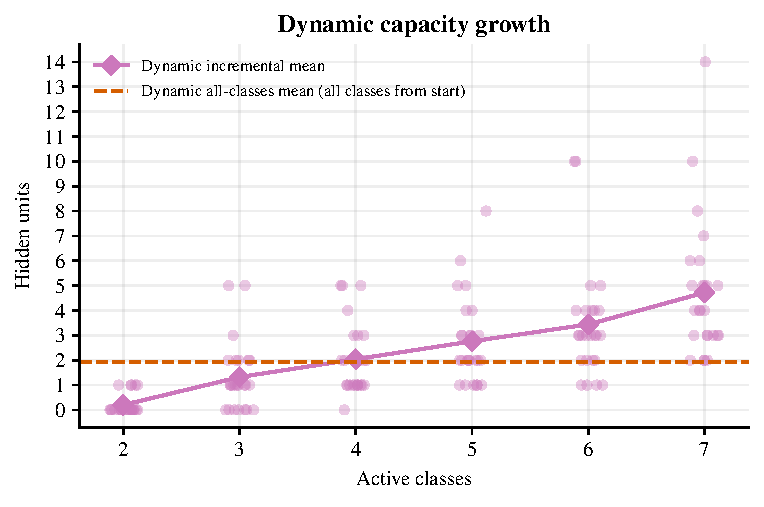
\includegraphics[width=.47\textwidth]{figures/dry_bean/network_growth.pdf}}\hfill
\subfloat[Steel Plates Faults]{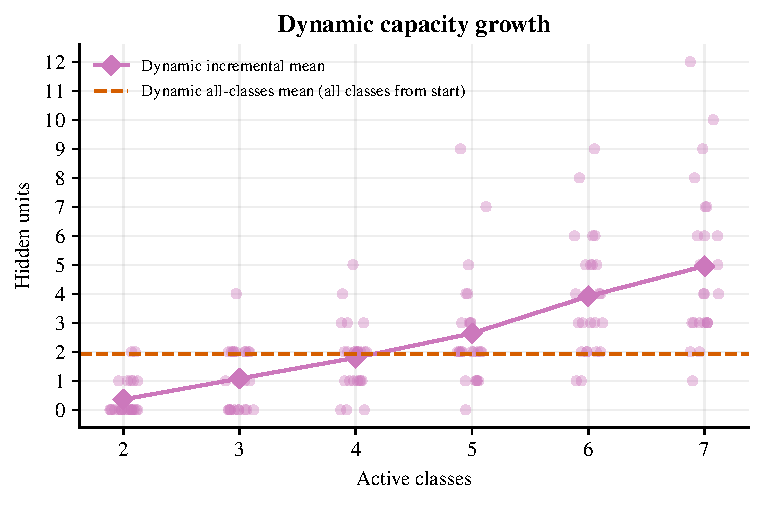
\includegraphics[width=.47\textwidth]{figures/steel_plates/network_growth.pdf}}
\caption{Validation-triggered hidden-capacity growth. Jittered points show all 25 fold and seed runs at each number of active classes; diamonds and their connecting line show stage means. The dashed line shows the dynamic all-classes mean across its 25 single-stage runs, with every class available from the start.}\label{fig:growth}
\end{figure*}
\begin{figure*}[t]\centering
\subfloat[Dry Bean]{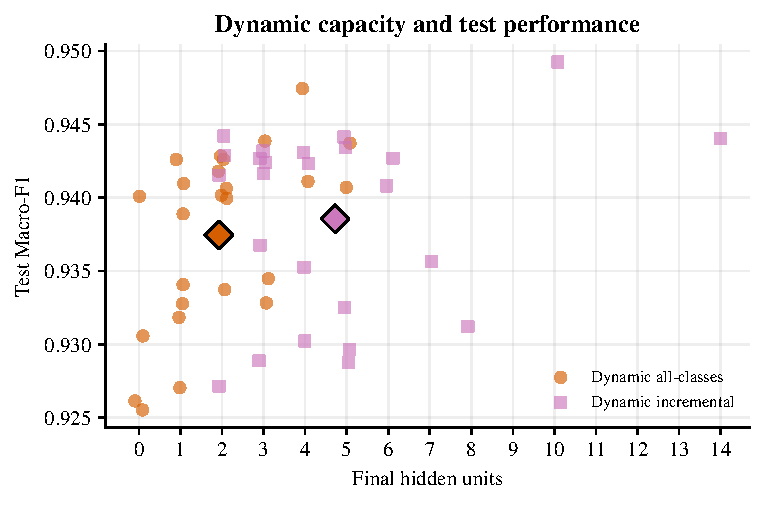
\includegraphics[width=.47\textwidth]{figures/dry_bean/dynamic_capacity_performance.pdf}}\hfill
\subfloat[Steel Plates Faults]{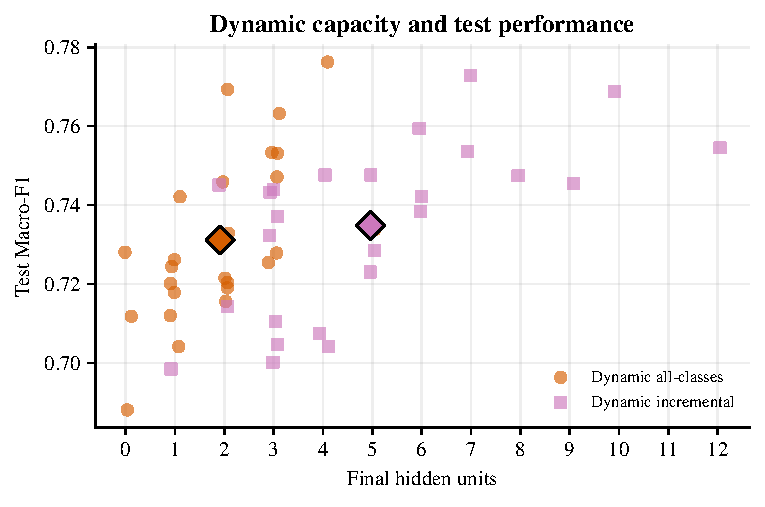
\includegraphics[width=.47\textwidth]{figures/steel_plates/dynamic_capacity_performance.pdf}}
\caption{Observed final hidden units and test Macro-F1 for each dynamic all-classes and dynamic incremental run. Horizontal jitter separates equal integer capacities; large diamonds show method means. Capacity is an outcome of growth, so the association is descriptive.}\label{fig:dynamic-capacity-performance}
\end{figure*}

\subsection{Computational Cost and Cross-Data-Set Comparison}
\begin{table*}[t]
\caption{Training cost: Dry Bean}
\label{tab:dry-bean-efficiency}
\centering\small
\resizebox{\textwidth}{!}{\begin{tabular}{lrrrrrr}
\toprule Method & Mean updates & Mean examples processed & Mean final hidden & Accepted & Rejected & Mean time (s)\\
\midrule
Ordinary baseline & 1766 & 225341 & 108.8 & 0.0 & 0.0 & 1.7\\
Fixed update-budget control & 3844 & 490365 & 108.8 & 0.0 & 0.0 & 3.7\\
Dynamic all-classes & 6798 & 867213 & 1.9 & 1.9 & 1.0 & 1.5\\
Dynamic incremental & 13279 & 1677827 & 4.7 & 4.7 & 6.0 & 3.6\\
Fixed incremental & 3844 & 485332 & 108.8 & 0.0 & 0.0 & 3.8\\
\bottomrule
\end{tabular}}
\end{table*}
\begin{table*}[t]
\caption{Training cost: Steel Plates Faults}
\label{tab:steel-plates-efficiency}
\centering\small
\resizebox{\textwidth}{!}{\begin{tabular}{lrrrrrr}
\toprule Method & Mean updates & Mean examples processed & Mean final hidden & Accepted & Rejected & Mean time (s)\\
\midrule
Ordinary baseline & 264 & 33341 & 320.0 & 0.0 & 0.0 & 0.9\\
Fixed update-budget control & 543 & 68508 & 320.0 & 0.0 & 0.0 & 1.7\\
Dynamic all-classes & 1274 & 160702 & 1.9 & 1.9 & 1.0 & 0.7\\
Dynamic incremental & 2009 & 233601 & 5.0 & 5.0 & 6.0 & 1.9\\
Fixed incremental & 543 & 62887 & 320.0 & 0.0 & 0.0 & 2.1\\
\bottomrule
\end{tabular}}
\end{table*}

The dynamic methods produced much smaller final networks than the fixed-capacity methods, but dynamic incremental required more gradient updates and processed more examples while attaining lower absolute Macro-F1 (Tables~\ref{tab:dry-bean-efficiency} and~\ref{tab:steel-plates-efficiency}; Fig.~\ref{fig:performance-cost}). Thus, under the canonical growth rule, compactness was accompanied by lower predictive performance rather than obtained without cost. Wall-clock times were nevertheless comparatively similar. This is consistent with each dynamic update operating on a much smaller network and with early curriculum stages using only a subset of classes, but the measured timings are environment-dependent and do not isolate either source of the difference.
\begin{figure*}[t]\centering
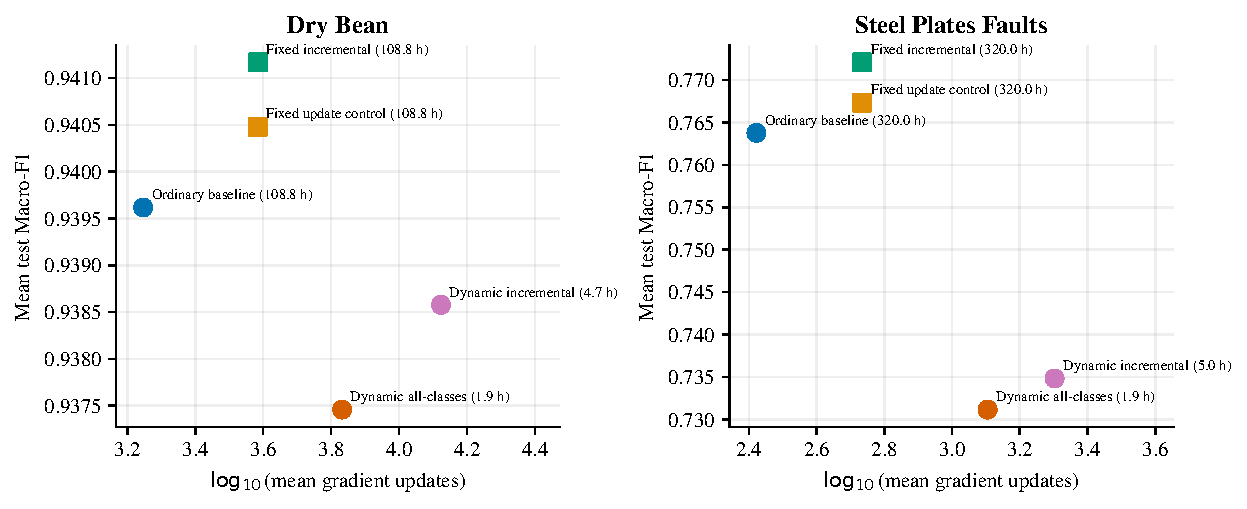
\includegraphics[width=.94\textwidth]{figures/performance_cost.pdf}
\caption{Descriptive performance and optimisation cost for five methods in each dataset. Points show mean test Macro-F1 against mean gradient updates on a logarithmic horizontal scale. Labels give mean final hidden units ($h$); symbol shapes distinguish fixed-capacity methods. The figure compares observed performance, effort, and size without implying a causal effect of any one quantity.}\label{fig:performance-cost}
\end{figure*}

Steel Plates was both more imbalanced and harder under the ordinary baseline than Dry Bean (Table~\ref{tab:data}; Tables~\ref{tab:dry-bean-overall} and~\ref{tab:steel-plates-overall}). Its curriculum point estimates were also larger, but the wider intervals and small number of folds do not support attributing that difference to imbalance or task difficulty (Tables~\ref{tab:dry-bean-statistics} and~\ref{tab:steel-plates-statistics}; Fig.~\ref{fig:primary-effects}). The heterogeneous class-level effects in Fig.~\ref{fig:per-class-effects} further show that the aggregate difference was not distributed uniformly across classes.

\subsection{Sensitivity and Limitations}
The validation-only sensitivity grid shows that plausible probe settings changed validation Macro-F1 by amounts comparable to or larger than the observed dynamic curriculum point estimates (Fig.~\ref{fig:sensitivity}; Tables~\ref{tab:dry-bean-statistics} and~\ref{tab:steel-plates-statistics}). Because these settings govern only the dynamic growth procedure, the dynamic conclusions should be interpreted as conditional on the chosen growth rule rather than as evidence for a generally robust adaptive-capacity effect. The grid used validation data and one optimisation seed, so it supports a limitation on robustness rather than an additional test-set claim.
\begin{figure*}[t]\centering
\subfloat[Dry Bean]{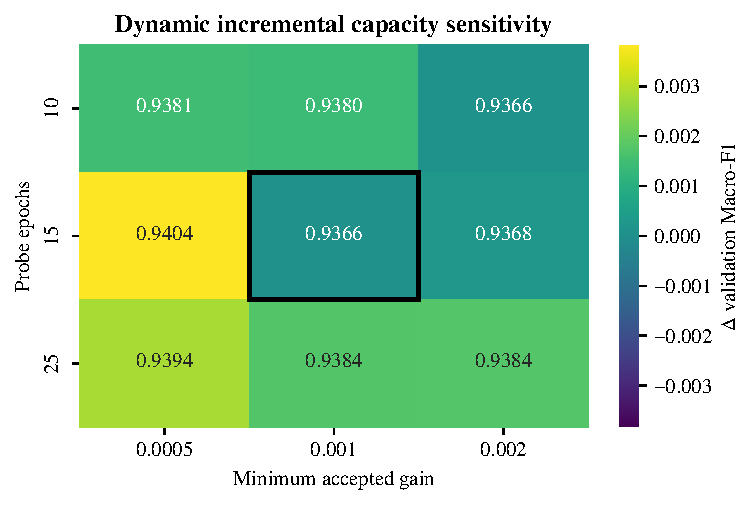
\includegraphics[width=.47\textwidth]{figures/dry_bean/capacity_sensitivity.pdf}}\hfill
\subfloat[Steel Plates Faults]{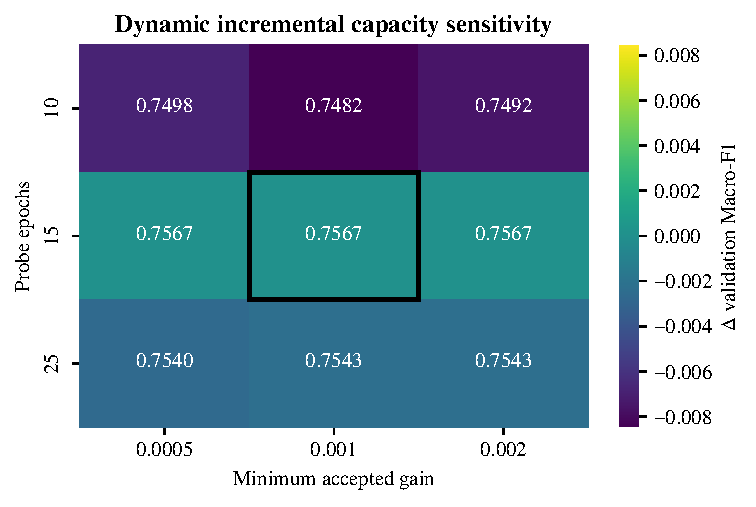
\includegraphics[width=.47\textwidth]{figures/steel_plates/capacity_sensitivity.pdf}}
\caption{Dynamic incremental validation-only capacity sensitivity. Colour shows change in mean validation Macro-F1 relative to the outlined canonical setting (15 probe epochs, minimum gain 0.001); cell text shows absolute mean validation Macro-F1. Each cell averages five inner validation partitions with one fixed optimisation seed. Panels use separate delta colour scales. No test outcomes entered setting selection.}\label{fig:sensitivity}
\end{figure*}

The findings cover two application domains and five test-fold estimates per domain. Outer training partitions overlapped, and the study used one optimiser and a residual classifier architecture. Elapsed times also depend on the execution environment. The intervals and corrected tests therefore support cautious statements about observed fold-level differences, not broad claims of a population-level benefit.

\clearpage
\section{Conclusion}
Fixed incremental learning had the highest observed overall and minority Macro-F1 means, but neither fixed nor dynamic controlled comparisons established a dependable effect of minority-first class order: every primary interval crossed zero (Tables~\ref{tab:dry-bean-statistics} and~\ref{tab:steel-plates-statistics}; Fig.~\ref{fig:primary-effects}). The fixed result therefore distinguishes highest observed performance from evidence that presentation order itself caused an improvement. Dynamic growth did adapt to the expanding task by increasing capacity across stages, yet the resulting networks remained far smaller than the fixed-capacity models and retained lower absolute Macro-F1 while requiring more optimisation (Figs.~\ref{fig:growth} and~\ref{fig:performance-cost}; Tables~\ref{tab:dry-bean-efficiency} and~\ref{tab:steel-plates-efficiency}). The stronger imbalance and larger point estimates on Steel Plates did not support a causal cross-dataset explanation, and conclusions remain limited by two datasets, five overlapping outer-training partitions, and sensitivity to the growth settings (Fig.~\ref{fig:sensitivity}).

\bibliographystyle{IEEEtran}
\setlength{\emergencystretch}{3em}\sloppy
\bibliography{references}
\end{document}
